\documentclass[10pt,a4paper]{amsart}
\usepackage[margin=19mm]{geometry}
\usepackage{amsmath,amssymb,mathtools}
\usepackage[scr=rsfs,cal=euler]{mathalfa}
\usepackage{xfrac}
\usepackage[unicode,hidelinks,bookmarks=false]{hyperref}
\newcommand{\ie}{i.e.\ }
\newcommand{\cf}{cf.\ }
\newcommand{\resp}{respectively\ }
\newcommand{\Subsection}{\subsection}
\providecommand{\nobreakdash}{\nobreak\hbox{-}}
\setlength{\emergencystretch}{2em}
\multlinegap0pt
\usepackage{tikz}
\usepackage{amssymb}
\usepackage[all]{xy}
\newtheorem{definition}{Definition}
\newtheorem{proposition}{Proposition}
\newtheorem{lemma}{Lemma}
\newtheorem{scope}{Scope}
\title{A combinatorial approach to Kontsevich's Swiss cheese conjecture}
\author{Florian De Leger}
\date{Source: arXiv:2512.20167v1 (CC BY 4.0)}
\begin{document}
\maketitle

\noindent\emph{Source and licence.} A combinatorial approach to Kontsevich's Swiss cheese conjecture. Version arXiv:2512.20167v1 (CC BY 4.0), distributed by arXiv under the Creative Commons Attribution 4.0 International licence, http://creativecommons.org/licenses/by/4.0/, as recorded in the arXiv licence metadata for this exact version and shown on the abstract page https://arxiv.org/abs/2512.20167v1. Full licence notice: \texttt{licenses/arxiv-2512.20167-CC-BY-4.0.txt}.\par\smallskip

\noindent\textit{Editorial scope.} Counted unit: the article's lemma lemmaexistencecomplexitymap (source0.tex lines 613--618). The article's complete original proof of it is delivered with it (source0.tex lines 620--692, one \texttt{proof} environment of 73 lines). No mathematics is written, repaired or re-derived: the statement and the proof are the article's own lines, in the article's own notation, and no retained line is substituted or re-flowed.  Retained uncounted as the source-local context the proof needs: lines 299--310; lines 495--516.  Nothing was omitted from any retained span, so the package carries no omission record.  No retained line contains a citation, so the wrapper carries no bibliography and no bibliography entry.  The retained lines contain the article's own diagram code, which the wrapper typesets with the standard tikz packages; no image file is delivered and the package declares no asset dependency.  Editorial formatting only, in addition: an AMS \texttt{amsart} preamble that restates the article's own declarations and macros used by the retained lines, namely the environments \texttt{definition}, \texttt{proposition}, \texttt{lemma}, \texttt{scope} on separate counters, together with the standard packages those lines need.  The retained environments print in this document as Definition 1, Proposition 1, Lemma 1, Scope 1 in order of appearance, whereas the article prints the same items with the numbering of its own full document.  The complete native source of the article as distributed in the arXiv e-print for this exact version is bundled unchanged as \texttt{sources/191543/source0.tex}.
\begin{definition}\label{definitionpplus}
	For a categorical operad $\mathcal{P}$, let $\mathcal{P}^+$ be the operad in $\mathrm{Set}$ whose:
	\begin{itemize}
		\item colours are operations of $\mathcal{P}$,
		\item for $(c_1,\ldots,c_k,c) \in C^{k+1}$, let
		\[
		\mathcal{P}^+(c_1,\ldots,c_k;c)
		\]
		be the set of combed $\mathcal{P}$-trees with linearly ordered set of vertices $\{v_1,\ldots,v_k\}$, such that the operation which decorates $v_i$ is $c_i$, together with an extra morphism from the target of this $\mathcal{P}$-tree to $c$,
		\item multiplication is given by inserting a $\mathcal{P}$-tree inside the vertex of another $\mathcal{P}$-tree, reordering the set of leaves (combing) and composing the extra morphisms.
	\end{itemize}
\end{definition}

\begin{proposition}\label{propositionswisscheeseplus}
	$\mathcal{P}_{sc}^+$ is the Swiss cheese type operad whose:
	\begin{itemize}
		\item set of colours is $B \sqcup C$, where $B$ is the set of operations of $\mathcal{P}$ and $C$ is the set of colours of $\mathcal{P}$,
		\item for $(c_1,\ldots,c_k,c) \in B^{k+1}$,
		\[
			\mathcal{P}_{sc}^+(c_1,\ldots,c_k;c) = \mathcal{P}_*^+(c_1,\ldots,c_k;c).
		\]
		\item for $(c_1,\ldots,c_k) \in (B \sqcup C)^k$ and $c \in C$,
		\[
		\mathcal{P}_{sc}^+(c_1,\ldots,c_k;c)
		\]
		is the category whose objects are black and white $\mathcal{P}$-trees with linearly ordered set of vertices and leaves $\{x_1,\ldots,x_k\}$ such that
		\begin{itemize}
			\item if $c_i \in B$, $x_i$ is a vertex and if $c_i \in C$, $x_i$ is a leaf,
			\item in both cases, $x_i$ is decorated with $c_i$,
			\item the root edge is decorated with $c$,
		\end{itemize}
		and morphisms are given by a morphism for each black vertex,
		\item multiplication is given either by grafting the root of a $\mathcal{P}$-tree to the leaf of another $\mathcal{P}$-tree or by inserting as in Definition \ref{definitionpplus}.
	\end{itemize}
\end{proposition}

\begin{lemma}\label{lemmaexistencecomplexitymap}
	There is a lax morphism of operads
	\begin{equation}\label{equationmapc}
		f: (\mathcal{K}_n)_{sc}^+ \to \mathcal{RK}_{n+1}.
	\end{equation}
\end{lemma}

\begin{proof}
	Recall from Proposition \ref{propositionswisscheeseplus} that the set of colours of $(\mathcal{K}_n)_{sc}^+$ is $B \sqcup 1$, where $\mathcal{B}$ is the set of operations of $\mathcal{K}_n$ and $1 = \{*\}$ is the singleton set. The set of operations of $\mathcal{RK}_{n+1}$ is $\{\mathsf{f},\mathsf{h}\}$. On colours, $f$ sends an element of $B$ to $\mathsf{f}$ and $*$ to $\mathsf{h}$.
	
	Now let $(c_1,\ldots,c_k,c) \in (B \sqcup 1)^{k+1}$ and let us define a functor
	\[
	f: (\mathcal{K}_n)_{sc}^+(c_1,\ldots,c_k;c) \to \mathcal{RK}_{n+1}(f(c_1),\ldots,f(c_k);f(c))
	\]
	Let $x \in (\mathcal{K}_n)_{sc}^+(c_1,\ldots,c_k;c)$. Let $f(x) := (\mu,\sigma)$, where $\mu$ and $\sigma$ are defined as follows. Recall that $x$ is a black and white $\mathcal{K}_n$-tree and each element $\{1,\ldots,k\}$ corresponds to a vertex or a leaf of this tree. For $1 \leq i < j \leq k$, if $i$ and $j$ are one above the other, then $\mu_{ij}:=n+1$ and
	\[
	\sigma_{ij} = 
	\begin{cases}
	id &\text{if $i$ is above $j$,} \\
	(12) &\text{if $i$ is below $j$.}
	\end{cases}
	\]
	If $i$ and $j$ are not one above the other, then there is a maximal vertex $v$ in the $\mathcal{K}_n$-tree $x$ which lies below $i$ and $j$. Note that $v$ is decorated with an operation $(\mu',\sigma') \in \mathcal{K}_n(|v|)$, where $|v|$ is the number of input edges of $v$. Let $l$ and $m$ in $\{1,\ldots,|v|\}$ corresponding to the edges that lie below $i$ and $j$ respectively. We define $(\mu_{ij},\sigma_{ij}) := (\mu'_{lm},\sigma'_{lm})$. As an illustration, the functor
	\begin{equation}\label{equationexamplecomplexitymap}
		f: (\mathcal{K}_2)_{sc}^+(*,*,c_3,c_4,*;*) \to \mathcal{RK}_3(\mathsf{h},\mathsf{h},\mathsf{f},\mathsf{f},\mathsf{h};\mathsf{h})
	\end{equation}
	can be pictured as follows:
	\[
	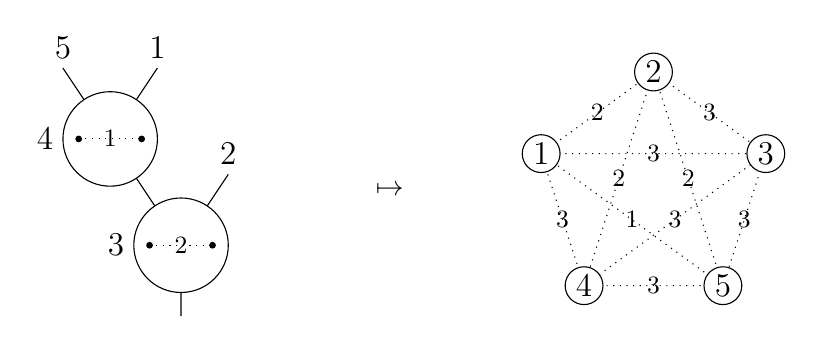
\begin{tikzpicture}
	\draw (0,-.9) -- (0,0) -- (-1.5,2.25) node[above]{\large{$5$}};
	\draw (0,0) -- (.6,.9) node[above]{\large{$2$}};
	\draw (-.9,1.35) -- (-.3,2.25) node[above]{\large{$1$}};
	\draw (-.6,0) node[left]{\large{$3$}};
	\draw (-1.5,1.35) node[left]{\large{$4$}};
	
	\draw[fill=white] (0,0) circle (.6);
	\draw[dotted] (-.4,0) -- (.4,0);
	\draw (0,0) node{\small{$2$}};
	\draw[fill] (-.4,0) circle (1pt);
	\draw[fill] (.4,0) circle (1pt);
	\draw[fill=white] (-.9,1.35) circle (.6);
	\draw[dotted] (-1.3,1.35) -- (-.5,1.35);
	\draw (-.9,1.35) node{\small{$1$}};
	\draw[fill] (-1.3,1.35) circle (1pt);
	\draw[fill] (-.5,1.35) circle (1pt);
	
	\draw (2.65,.7) node{$\mapsto$};
	
	\begin{scope}[shift={(6,.7)},scale=1.5]
	\draw[dotted] ({cos(54)},{-sin(54)}) -- ({cos(18)},{sin(18)}) -- (0,1) -- ({-cos(18)},{sin(18)}) -- ({-cos(54)},{-sin(54)}) -- ({cos(54)},{-sin(54)}) -- (0,1) -- ({-cos(54)},{-sin(54)}) -- ({cos(18)},{sin(18)}) -- ({-cos(18)},{sin(18)}) -- ({cos(54)},{-sin(54)});
	
	\draw[fill=white] ({cos(18)},{sin(18)}) circle (.16) node{\large{$3$}};
	\draw[fill=white] (0,1) circle (.16) node{\large{$2$}};
	\draw[fill=white] ({-cos(18)},{sin(18)}) circle (.16) node{\large{$1$}};
	\draw[fill=white] ({-cos(54)},{-sin(54)}) circle (.16) node{\large{$4$}};
	\draw[fill=white] ({cos(54)},{-sin(54)}) circle (.16) node{\large{$5$}};
	
	\draw (0,{-sin(54)}) node{\small{$3$}};
	\draw ({cos(18)/2+cos(54)/2},{sin(18)/2-sin(54)/2}) node{\small{$3$}};
	\draw ({cos(18)/2},{sin(18)/2+1/2}) node{\small{$3$}};
	\draw ({-cos(18)/2},{sin(18)/2+1/2}) node{\small{$2$}};
	\draw ({-cos(18)/2-cos(54)/2},{sin(18)/2-sin(54)/2}) node{\small{$3$}};
	\draw ({cos(18)/2-cos(54)/2},{sin(18)/2-sin(54)/2}) node{\small{$3$}};
	\draw (0,{sin(18)}) node{\small{$3$}};
	\draw ({cos(54)/2-cos(18)/2},{sin(18)/2-sin(54)/2}) node{\small{$1$}};
	\draw ({cos(54)/2},{1/2-sin(54)/2}) node{\small{$2$}};
	\draw ({-cos(54)/2},{1/2-sin(54)/2}) node {\small{$2$}};
	\end{scope}
	\end{tikzpicture}
	\]
	$c_3$ and $c_4$ in \eqref{equationexamplecomplexitymap} are the operations which decorate the vertices numbered by $3$ and $4$ respectively.
	
	Note that if $i$ and $j$ satisfy one of the following:
	\begin{itemize}
		\item $f(c_i)=f(c_j)=\mathsf{h}$,
		\item $f(c_i)=\mathsf{f}$, $f(c_j)=\mathsf{h}$ and $\sigma_{ij}=id$,
		\item $f(c_i)=\mathsf{h}$, $f(c_j)=\mathsf{f}$ and $\sigma_{ij}=(12)$,
	\end{itemize}
	then, since nothing can be above a leaf, $i$ and $j$ can not be one above the other, so $\mu_{ij} \leq n$. This proves that $f$ is well-defined. The proof that $f$ is indeed a lax morphism of operads is left to the reader.
\end{proof}

\end{document}
